\chapter{SatNOGS: Глобальная сеть наземных спутниковых станций с открытым исходным кодом}

SatNOGS представляет собой комплексную платформу \cite{satnogs_general_docs},
обеспечивающую функционирование открытой сети наземных станций для мониторинга
спутников. Основной целью проекта является разработка полного стека открытых
технологий, основанных на открытых стандартах, и создание полноценной наземной
станции в качестве демонстрации возможностей данного стека.

Система SatNOGS способна принимать сигналы со спутников, находящихся на низкой
околоземной орбите (LEO), в диапазонах UHF и VHF. Она позволяет извлекать
сигналы состояния и телеметрии, данные с научных и исследовательских спутников
(например, результаты магнитосферных экспериментов), метеорологические данные и
другую информацию.

Проект SatNOGS включает в себя несколько ключевых компонентов: веб-приложение
для планирования наблюдений, базу данных для хранения информации о спутниках,
клиентское программное обеспечение для работы на наземных станциях и аппаратное
обеспечение с открытым исходным кодом. Все это создает модульную архитектуру,
позволяющую легко интегрировать новые функции и расширять функциональность
системы.

SatNOGS активно развивает сообщество пользователей и разработчиков, предлагая
доступ к документации и инструментам для создания собственных наземных станций.
Это создает возможности для участия в глобальной сети наблюдений за спутниками
и обмена данными между участниками проекта.

\section{Текущее состояние сети SatNOGS}

Сеть SatNOGS, запущенная в 2015 году, трансформировалась из небольшого
экспериментального проекта в масштабную глобальную инфраструктуру наблюдения за
спутниками. За относительно короткий период своего существования проект
продемонстрировал значительный рост как в количественном, так и в качественном
отношении.

\subsection{Динамика развития сети}

Экспоненциальный рост сети SatNOGS обусловлен несколькими ключевыми факторами.
Возрастающая популярность малых спутников формата CubeSat в сочетании с
открытой архитектурой платформы способствовали стремительному увеличению числа
активных наземных станций. Параллельно с количественным ростом происходило и
качественное развитие экосистемы, включающее внедрение систем автоматического
декодирования телеметрии и инструментов визуального анализа спектра, что
существенно расширило функциональные возможности сети.

\subsection{Количественные показатели функционирования}

Текущая операционная активность сети характеризуется следующими показателями:

\begin{table}[h]
	\centering
	\begin{tabular}{|l|c|}
		\hline
		\textbf{Параметр}                                   & \textbf{Значение} \\
		\hline
		Ежедневные наблюдения                               & $\sim$1200        \\
		Доля качественных наблюдений                        & 70\%              \\
		Ежедневный прирост декодированных кадров телеметрии & $\sim$2500        \\
		\hline
	\end{tabular}
	\caption{Основные операционные показатели сети SatNOGS}
	\label{tab:satnogs_stats}
\end{table}

Особенно примечателен рост количества ежедневных наблюдений: от нескольких
десятков в начальный период до более тысячи в настоящее время. Качество
получаемых данных также поддерживается на высоком уровне, с преобладанием
полезных наблюдений над классифицированными как "плохие" (содержащие помехи или
неполные данные) или "неудачные" (с техническими проблемами при загрузке).

\subsection{Фундаментальные принципы и перспективы развития}

В основе проекта SatNOGS лежат принципы открытости и доступности технологий.
Философия открытого программного и аппаратного обеспечения делает спутниковые
наблюдения доступными широкому кругу энтузиастов независимо от их технического
опыта и ресурсов. Сообщество, объединяющее радиолюбителей, инженеров,
исследователей и энтузиастов космоса, играет ключевую роль в развитии проекта.

Стратегические направления дальнейшего развития SatNOGS включают:

\begin{itemize}
	\item Внедрение методов машинного обучения для автоматизации верификации данных
	\item Оптимизацию алгоритмов планирования наблюдений для максимально эффективного использования ресурсов сети
	\item Расширение аналитических возможностей, включая предоставление необработанных данных для научных исследований
\end{itemize}

\subsection{Вклад в развитие космических исследований}

Значение SatNOGS для сообщества исследователей космоса многогранно. Проект
предоставляет инфраструктуру для приема и декодирования данных с малых
спутников, способствует развитию практических навыков в области радиотехники и
обработки сигналов, поддерживает научные и образовательные инициативы, а также
содействует демократизации космических технологий~\cite{satnogs_general_docs}.

\section{Компоненты SatNOGS}

SatNOGS включает в себя несколько ключевых компонентов, каждый из которых
играет важную роль в функционировании платформы, см. рисунок
\ref{fig:satnogs_data_flow}.
Ниже представлена таблица, описывающая основные элементы системы:

\begin{table}[h]
	\centering
	\begin{tabular}{|l|p{10cm}|}
		\hline \textbf{Компонент} & \textbf{Описание}
		\\ \hline SatNOGS Network          & Веб-приложение, предназначенное для
		планирования наблюдений по сети наземных станций. Оно способствует
		координации наблюдений за спутниковыми сигналами и планированию таких
		наблюдений среди наземных станций, подключенных к сети.                                 \\ \hline База
		данных SatNOGS            & Ресурс, позволяющий пользователям предоставлять
		информацию о передатчиках активных спутников. Данные доступны через API или
		веб-интерфейс.
		\\ \hline Клиент SatNOGS           & Программное обеспечение, работающее на
		наземных станциях (обычно на встраиваемых системах). Оно получает
		регулярные задания на наблюдение из сети, принимает спутниковые передачи и
		отправляет их обратно в веб-приложение Network.                                         \\ \hline Наземная станция
		SatNOGS                   & Аппаратное обеспечение наземной станции с открытым исходным
		кодом, включающее ротаторы, антенны и электронику, подключенные к клиенту.
		\\ \hline SatNOGS Dashboard        & Веб-интерфейс для визуализации и
		анализа данных телеметрии, полученных от спутников. Он предоставляет
		пользователям возможность отслеживать состояние спутников и их сигналы в
		реальном времени.                                                                       \\ \hline
	\end{tabular}
	\caption{Основные компоненты системы SatNOGS}
	\label{tab:satnogs_components}
\end{table}

Система SatNOGS активно развивает сообщество пользователей и разработчиков,
предлагая доступ к документации и инструментам для создания собственных
наземных станций. Это создает возможности для участия в глобальной сети
наблюдений за спутниками и обмена данными между участниками проекта.

\begin{figure}[htbp]
	\centering
	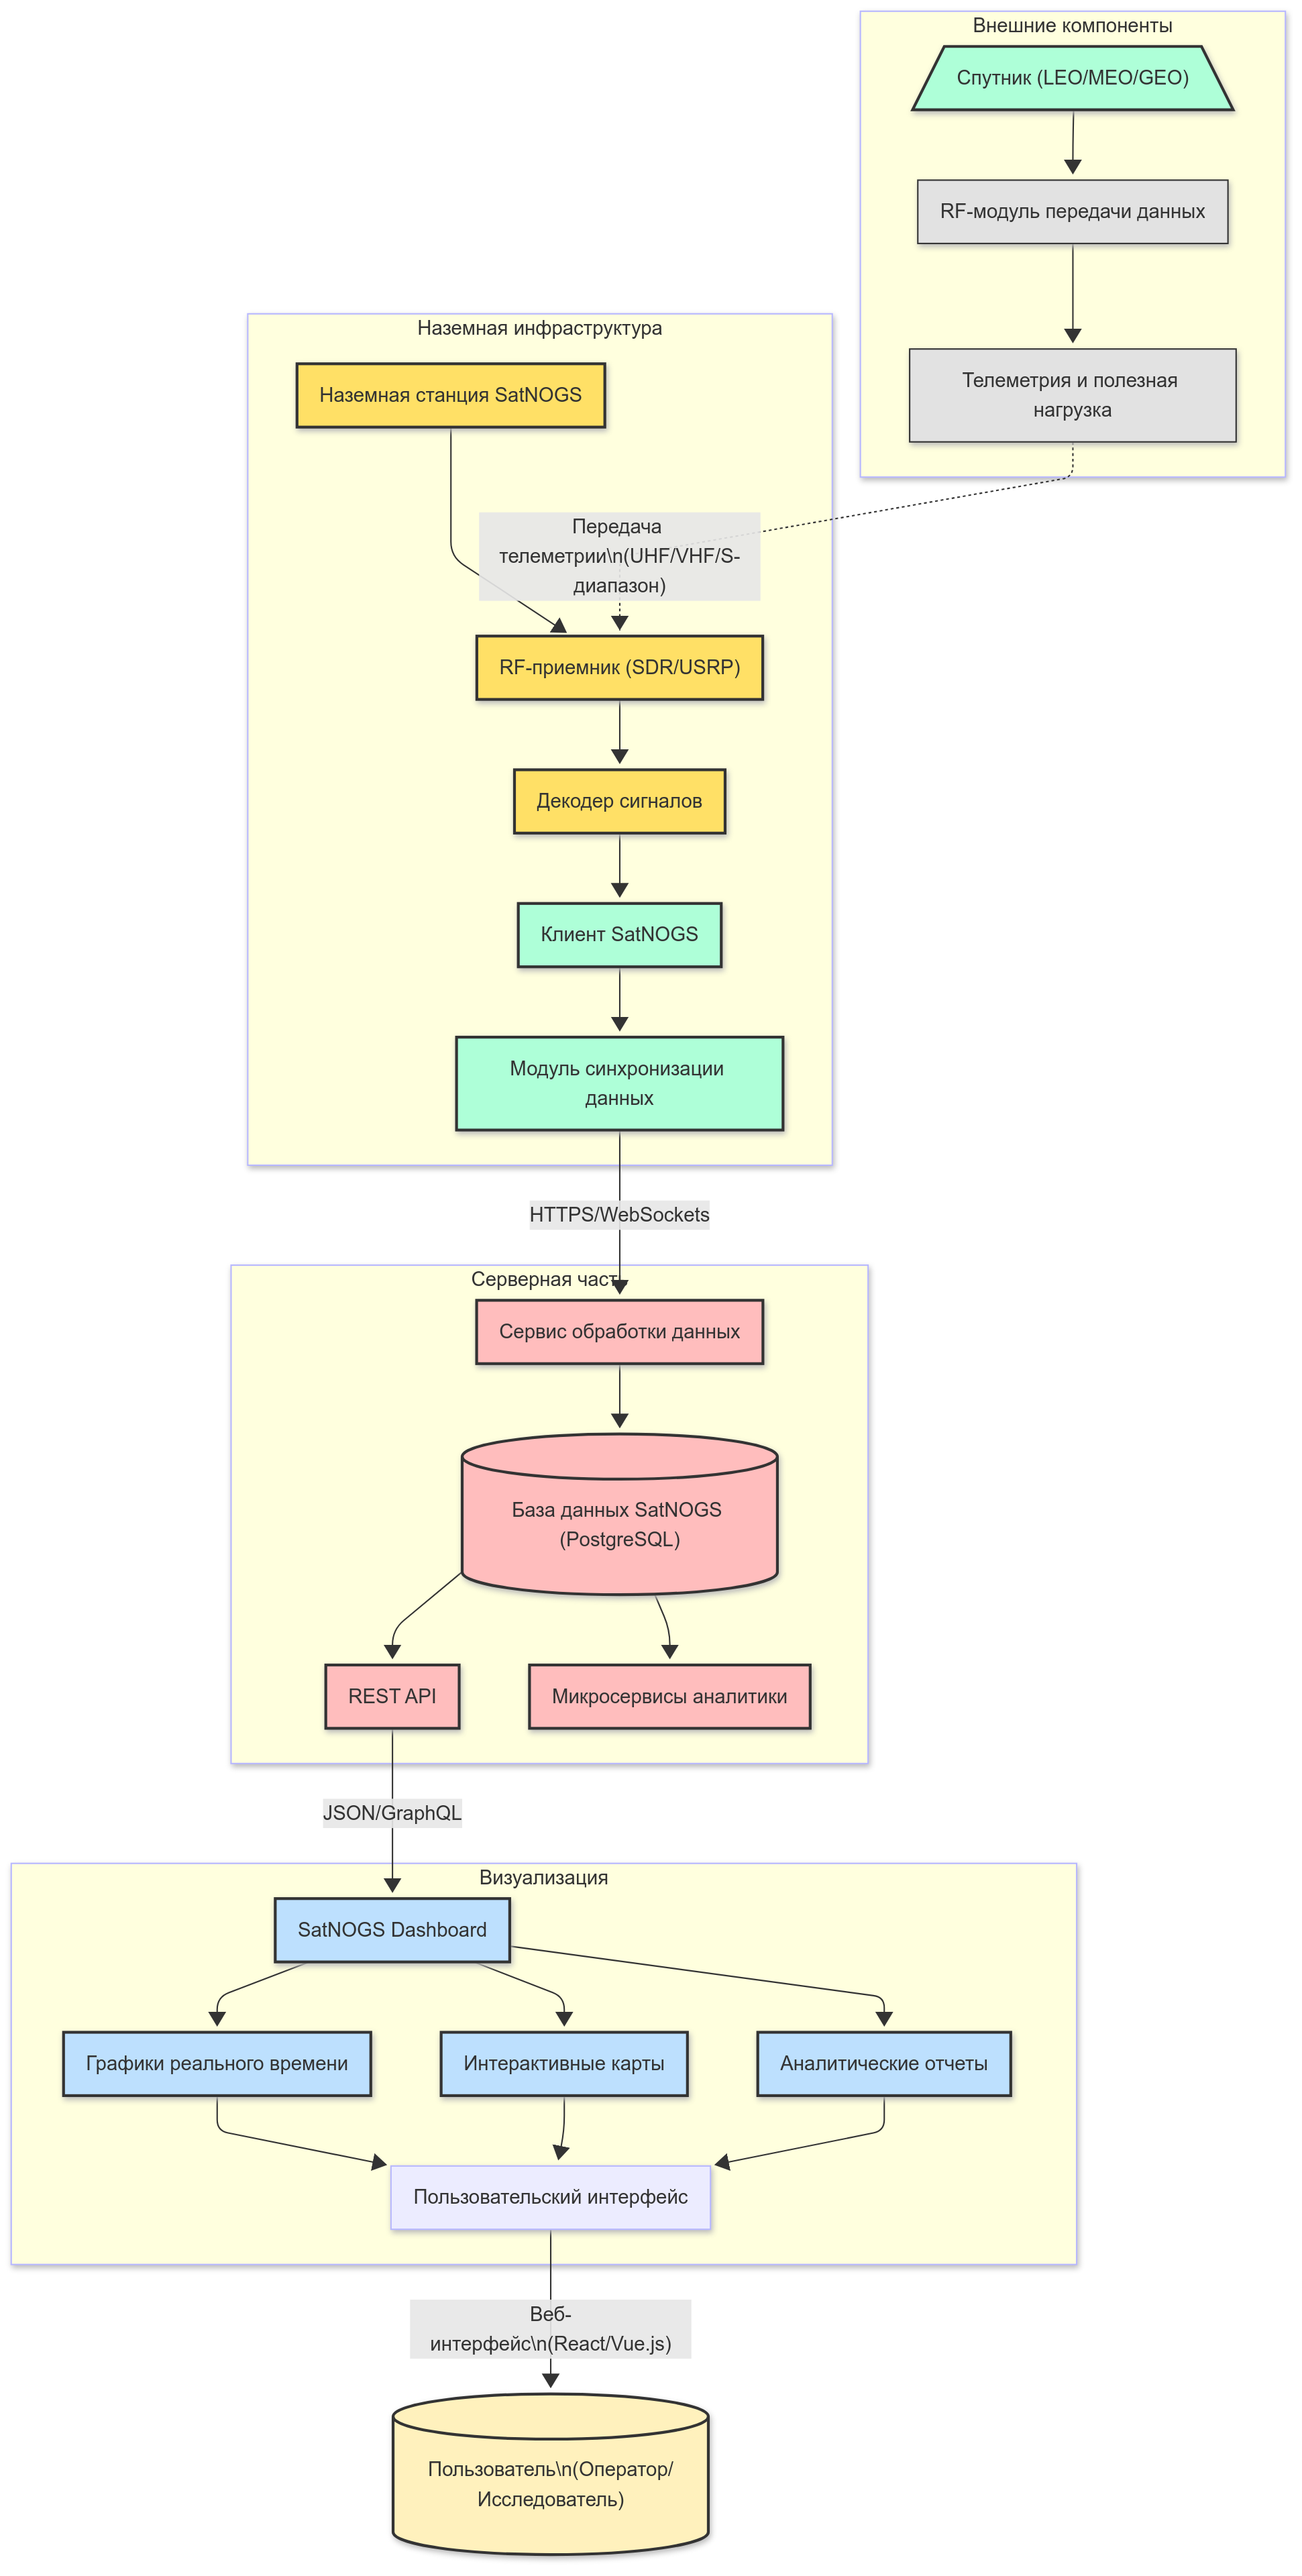
\includegraphics[width=0.7\textwidth]{satnogs_data_flow}
	\caption{Поток данных SatNOGS в Dashboard endpoint}
	\label{fig:satnogs_data_flow}
\end{figure}

\section{SatNOGS Dashboard}

\begin{figure}[htbp]
	\centering
	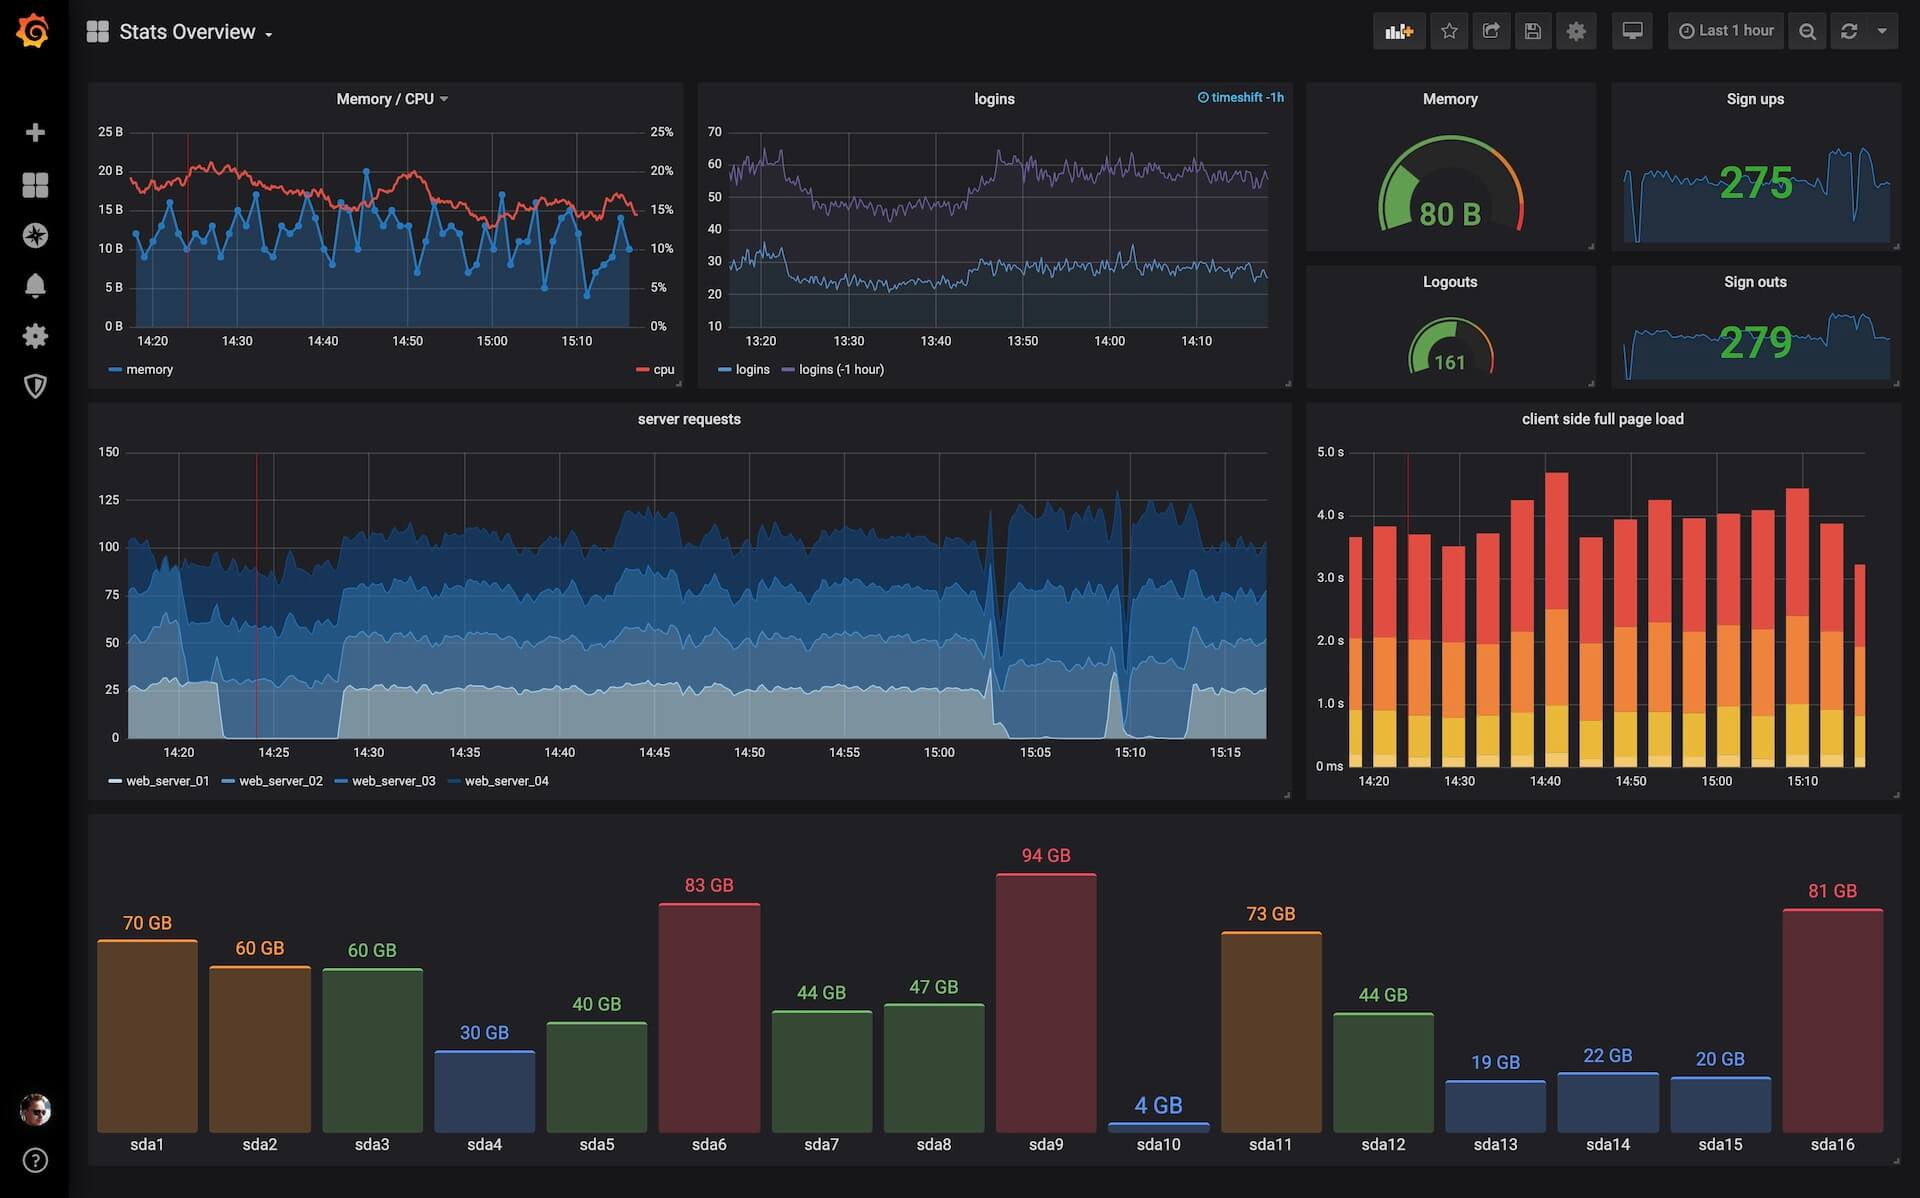
\includegraphics[width=1.0\textwidth]{grafana_example}
	\caption{Пример страницы с данными в Grafana Enterprise}
	\label{fig:grafana_example}
\end{figure}

SatNOGS Dashboard представляет собой ключевой компонент в нашей
исследовательской работе, выступая в качестве основного источника данных для
обучения моделей. После детального анализа архитектуры системы было определено
оптимальное место для извлечения данных. Dashboard Grafana в рамках экосистемы
SatNOGS предоставляет уже предобработанные данные, прошедшие фильтрацию и
дедупликацию посредством построения временных рядов. Несмотря на то, что
система содержит информацию только о приблизительно 120 спутниках, этот объем
является достаточным для анализа критических метрик и позволяет существенно
сократить затраты времени и вычислительных ресурсов на обучение, при этом
обеспечивая независимость от инфраструктуры SatNOGS.

Grafana — это мощная платформа для визуализации и анализа данных, которая
позволяет создавать интерактивные дашборды на основе различных источников
данных \cite{grafana_docs}. Пример такого дашборда можно увидеть на рисунке
\ref{fig:grafana_example}.
Grafana широко используется для мониторинга систем и приложений, предоставляя
пользователям возможность отслеживать ключевые метрики в реальном времени.

В контексте SatNOGS Dashboard, Grafana работает с базой данных
\textbf{InfluxDB} \cite{influxdb_docs}, которая предназначена для хранения
временных рядов данных, таких как телеметрия спутников. Данные поступают от
наземных станций, обрабатываются клиентом SatNOGS и сохраняются в InfluxDB.
Затем Grafana использует API для доступа к этим данным и их визуализации на
дашбордах.

Однако стоит отметить, что доступ к API Grafana Dashboard SatNOGS был закрыт,
что ограничивает возможности пользователей в получении данных напрямую. Более
того, Grafana не предоставляет свои услуги пользователям из России и Беларуси в
связи с санциями \cite{grafana_community_post}, что создает дополнительные
сложности для разработчиков и исследователей из этих стран. Это делает Grafana
ненадежной платформой для работы в нашем регионе.

В ответ на эти ограничения нами разрабатывается специализированный парсер для
обхода существующих барьеров и получения необходимых данных. Данный инструмент
будет подробно рассмотрен в последующих разделах работы, поскольку он является
ключевым компонентом для интеграции данных из SatNOGS Dashboard в нашу систему
анализа и визуализации.

Таким образом, несмотря на значительный потенциал Grafana как инструмента
визуализации, текущие ограничения доступа существенно снижают её практическую
ценность для пользователей из определённых регионов, что обуславливает
необходимость разработки альтернативных методов работы с данными.
Схему работы SatNOGS Dashboard можно наблюдать на рисунке
\ref{fig:grafana_infra}.

\begin{figure}[htbp]
	\centering
	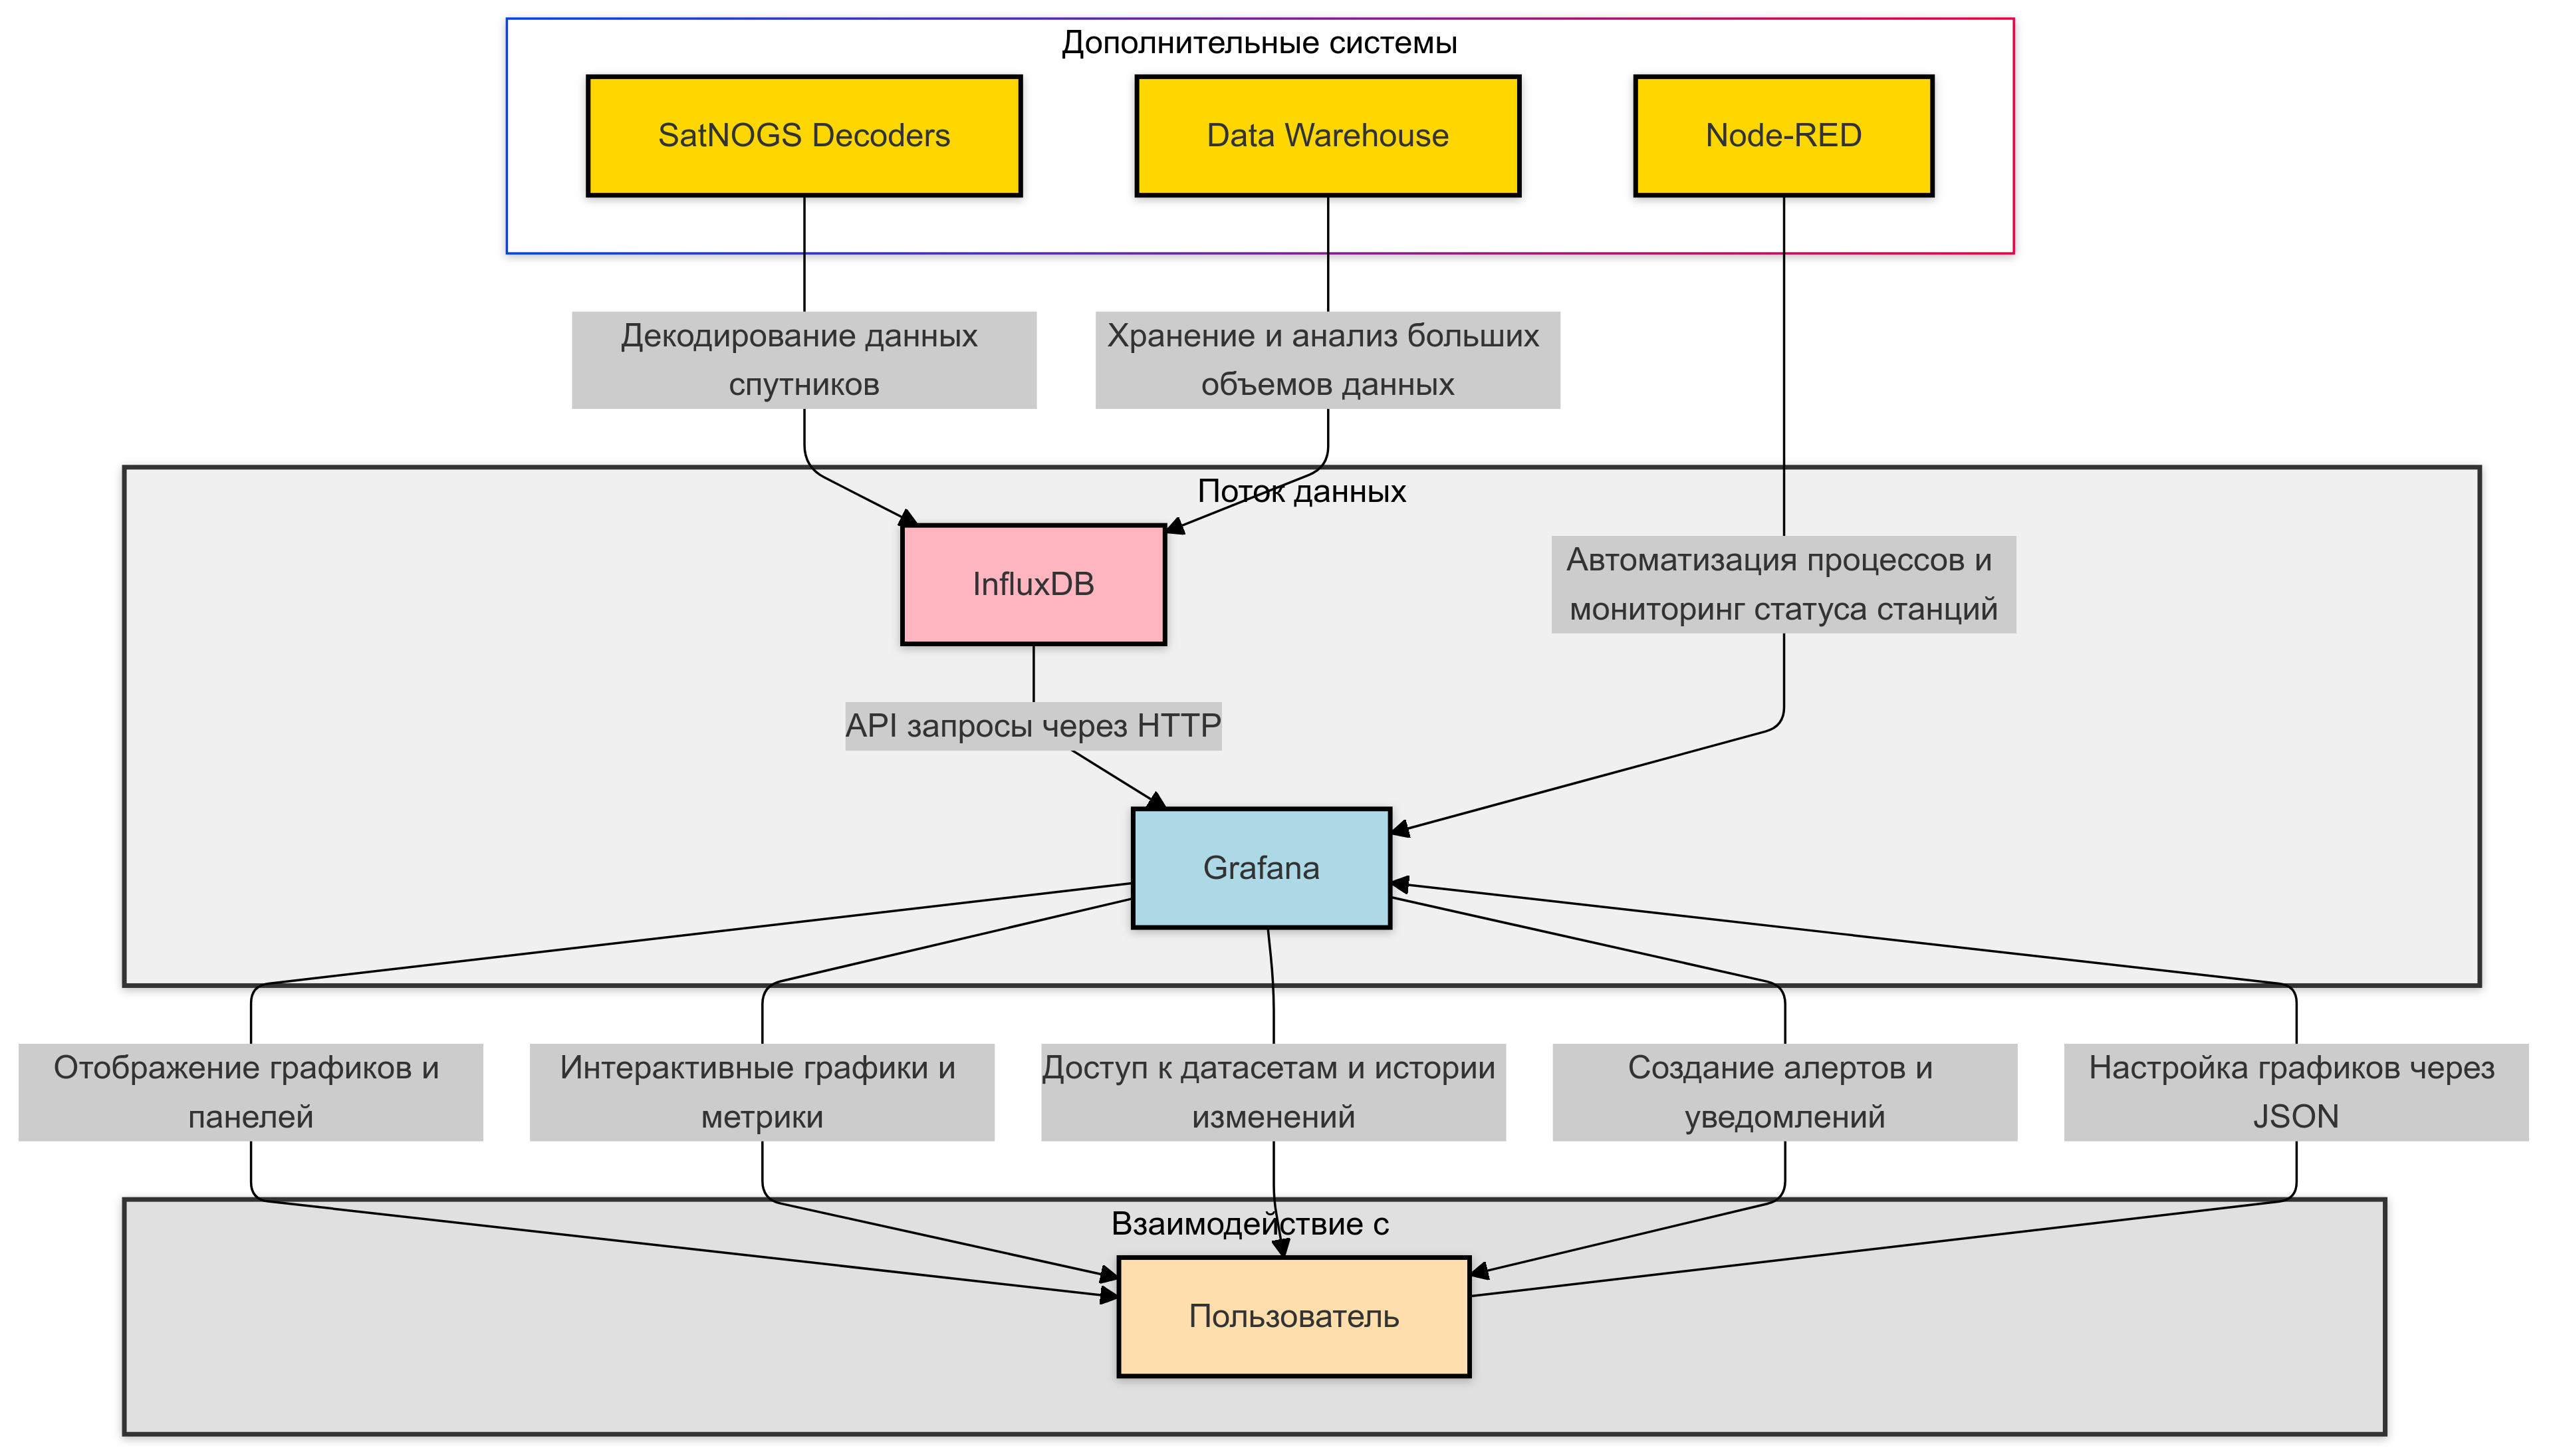
\includegraphics[width=1.0\textwidth]{grafana_infra}
	\caption{Подробное устройство SatNOGS Dashboard}
	\label{fig:grafana_infra}
\end{figure}

\subsection{Структура фронтенд-компонентов Grafana SatNOGS Dashboard}

\begin{figure}[htbp]
	\centering
	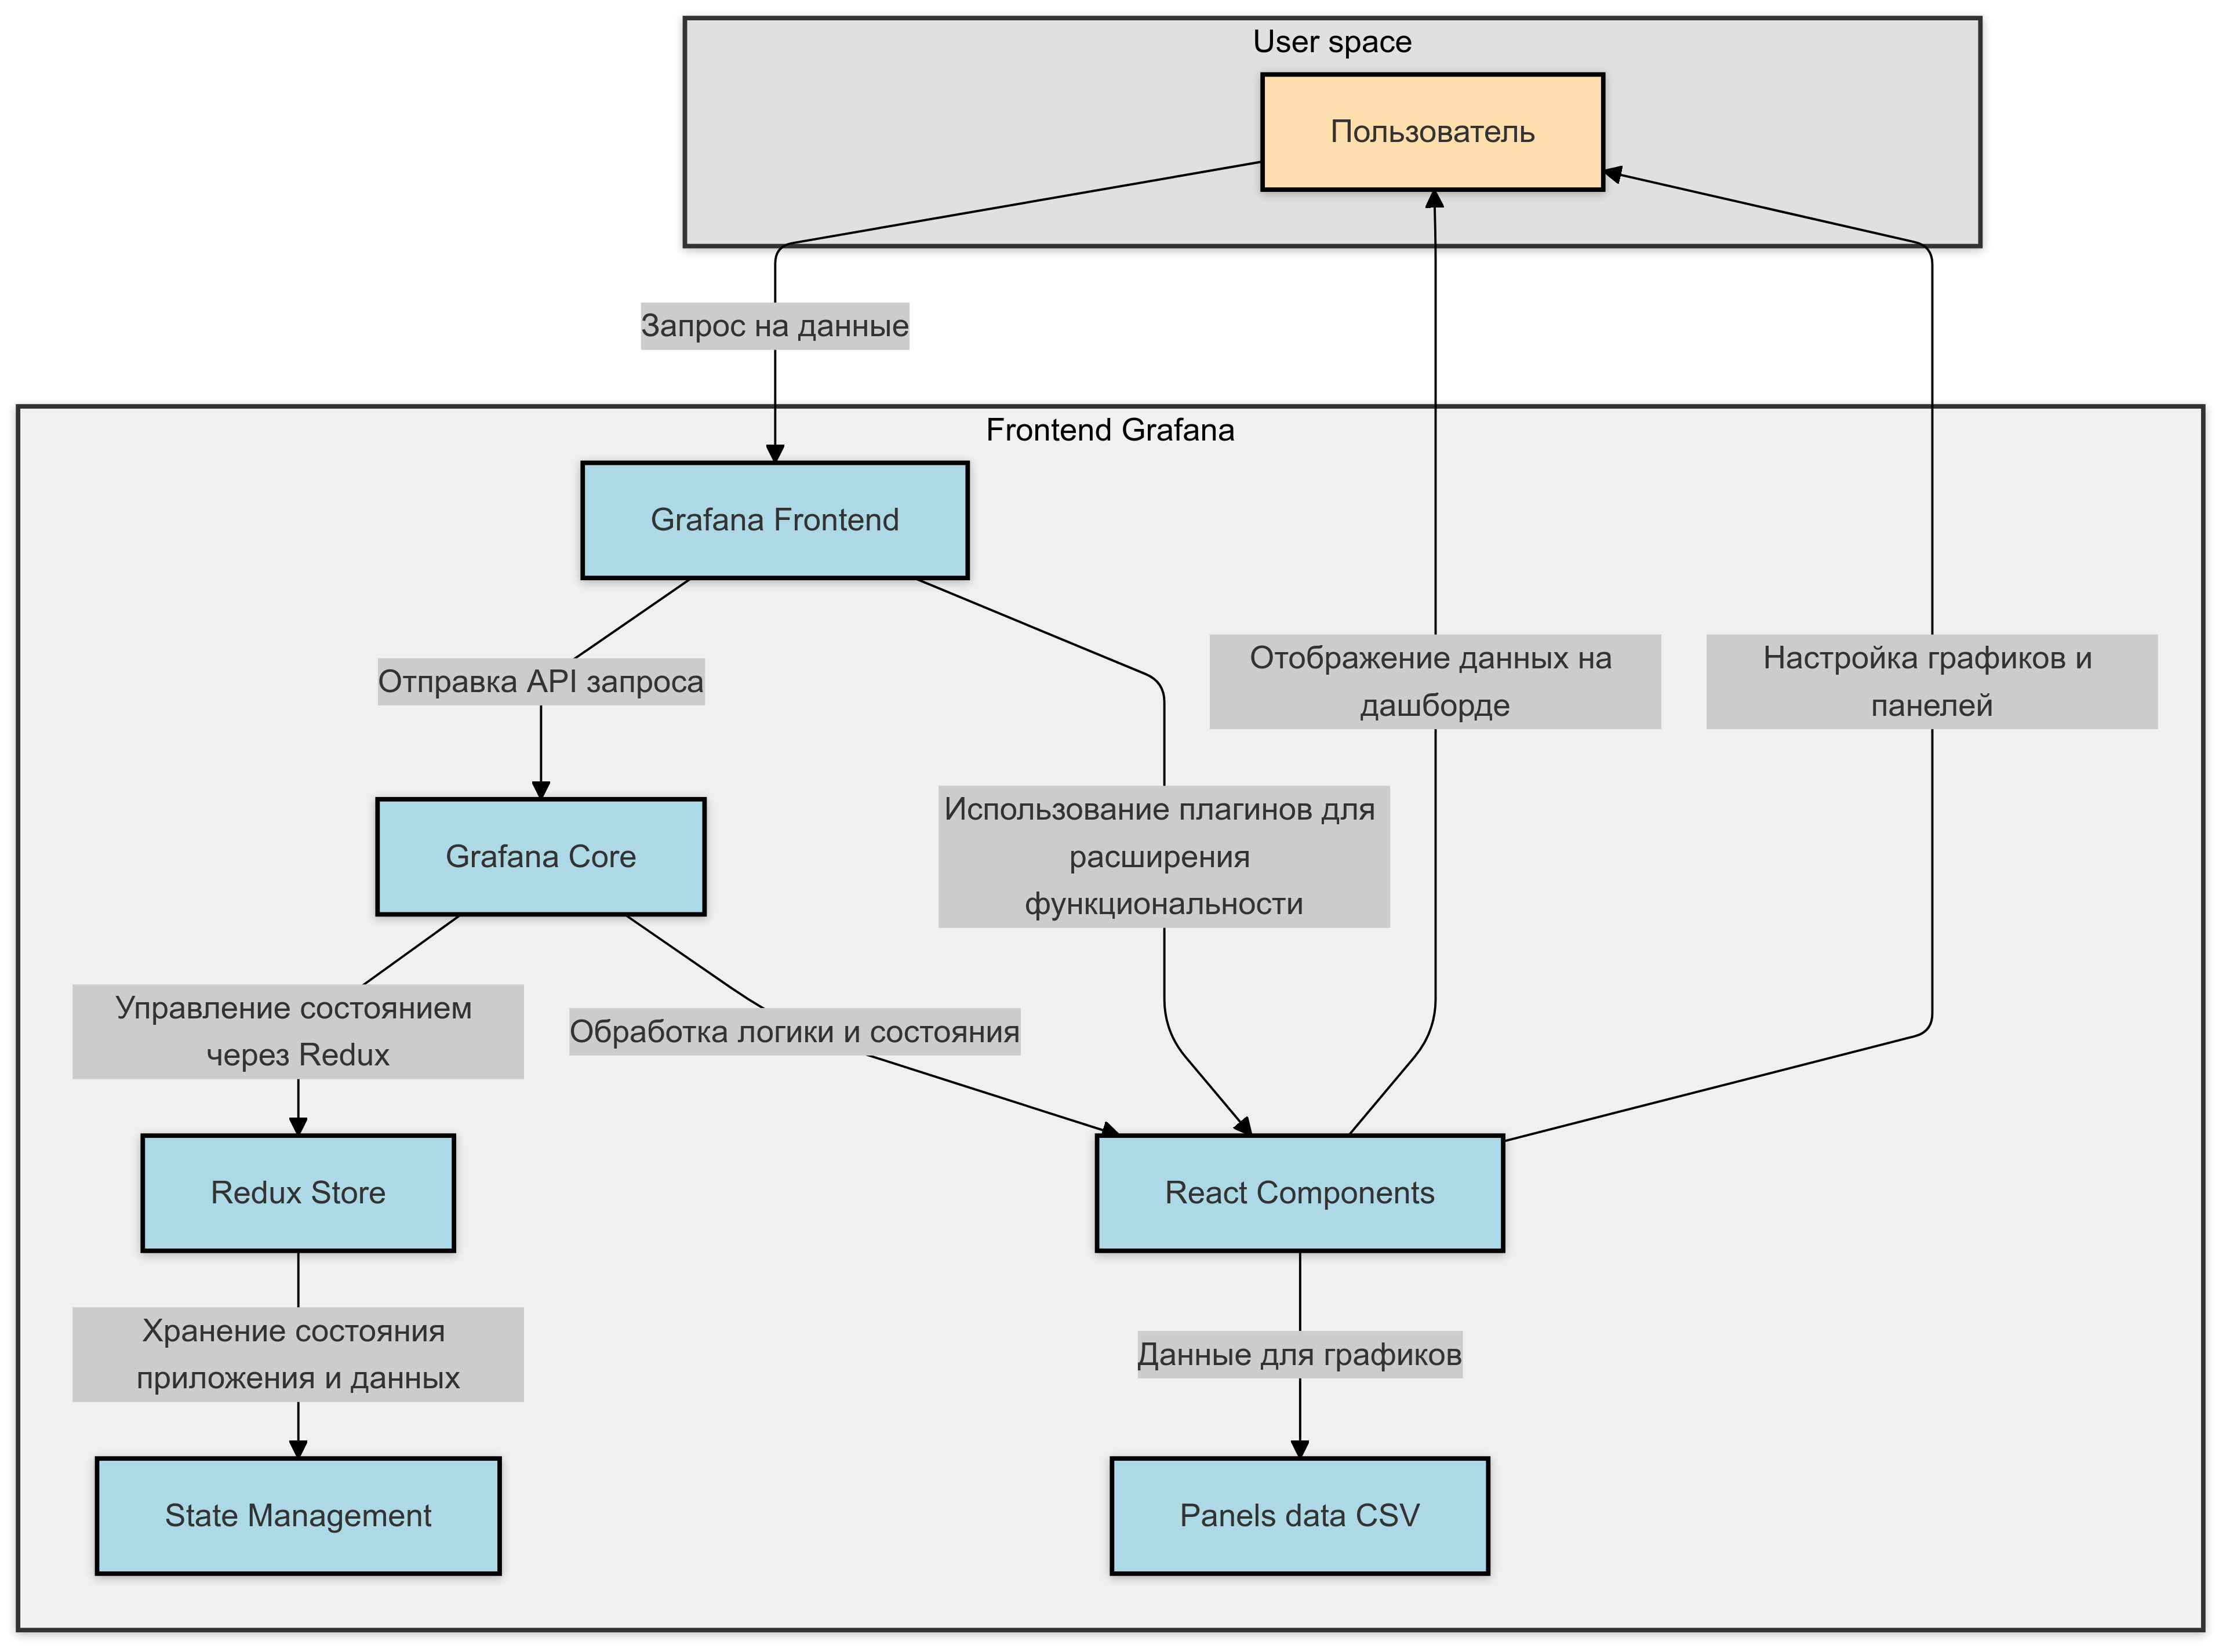
\includegraphics[width=1.0\textwidth]{grafana_frontend_structure}
	\caption{Построение frontend части grafana \cite{react_managing_state}}
	\label{fig:grafana_frontend_structure}
\end{figure}

Архитектура фронтенд-части Grafana
(рис.~\ref{fig:grafana_frontend_structure})
построена по многоуровневому принципу, где пользовательское пространство (User
space) взаимодействует с системой через запросы на получение данных. Фронтенд
Grafana включает несколько ключевых компонентов: Grafana Frontend, Grafana
Core, Redux Store, State Management, React Components и Panels data CSV.

Процесс обработки данных начинается с пользовательского запроса, который
принимается компонентом Grafana Frontend. Этот компонент формирует API-запросы
к Grafana Core, отвечающему за обработку бизнес-логики и управление состоянием
приложения. Grafana Core взаимодействует с Redux Store, реализующим паттерн
единого источника истины для централизованного управления состоянием.

Компонент State Management обеспечивает структурированное хранение данных о
конфигурации панелей, пользовательских настройках и результатах запросов. React
Components представляют презентационный слой системы, отвечая за визуализацию
данных на дашбордах и интерактивное взаимодействие с пользователем.

Особую роль в системе играет компонент Panels data CSV, который обрабатывает и
форматирует данные для последующей визуализации. Именно этот компонент является
ключевой точкой для извлечения структурированной информации при парсинге
системы.

\subsection{Веб скраппер данных grafana dashboard}

Система извлечения данных из Grafana использует многоуровневый подход для
эффективного сбора и обработки информации с панелей мониторинга. Ключевые
компоненты системы включают механизмы парсинга URL, асинхронной загрузки данных
и параллельной обработки информации.

Основной процесс извлечения данных реализован через последовательность
взаимосвязанных функций. Функция \texttt{parse\_grafana\_url} анализирует URL
панели Grafana, извлекая базовый URL и временной диапазон. Это обеспечивает
корректное формирование запросов с сохранением временного контекста. Функция
\texttt{build\_inspection\_url} создает специализированные URL для доступа к
данным конкретных панелей, включая необходимые параметры времени и
идентификаторы.

Для взаимодействия с интерфейсом Grafana используется асинхронная загрузка
JavaScript кода через функцию \texttt{\_load\_script}. Эти скрипты выполняются в
контексте браузера, извлекая список панелей и инициируя загрузку данных.
Полученные CSV файлы обрабатываются функцией \texttt{\_process\_csv}, которая
выполняет нормализацию временных меток, преобразование единиц измерения,
фильтрацию и переименование колонок для обеспечения совместимости.

Функция \texttt{\_download\_panel} запускает процесс загрузки данных для
конкретной панели, а \texttt{\_process\_panel} координирует весь процесс
обработки, включая навигацию, загрузку и сохранение результатов. Параллельное
извлечение данных организовано через функцию \texttt{\_scrape\_panels}, которая
обеспечивает обработку множества панелей пакетами с контролем конкурентности.

Техническая реализация системы основана на асинхронном программировании с
использованием asyncio, что позволяет эффективно обрабатывать множество
запросов параллельно. Применяются раздельные пулы потоков для операций
ввода-вывода и вычислений, что оптимизирует использование системных ресурсов.
Для снижения риска блокировки со стороны сервера используется регулирование
трафика через случайные задержки между запросами и обработку панелей пакетами.
Комплексная система обработки исключений обеспечивает устойчивость к сбоям, а
использование pandas позволяет эффективно трансформировать данные с применением
векторизованных операций.

Основное преимущество данного подхода заключается в его способности обходить
ограничения стандартного API путем эмуляции взаимодействия пользователя с
интерфейсом. Это позволяет получать данные даже в случаях, когда прямой доступ
к API ограничен или недоступен.

В контексте работы с SatNOGS Dashboard данный скрипт представляет собой
ключевой инструмент для получения телеметрических данных спутников, необходимых
для дальнейшего анализа и обучения моделей. Его применение позволяет преодолеть
ограничения доступа к данным и обеспечить независимость исследовательской
работы от внешней инфраструктуры.
